\documentclass{article}
\usepackage[left=1.5cm, right=2cm]{geometry}
\usepackage{makecell}
\usepackage{amsmath}
\usepackage{graphicx}
\renewcommand{\arraystretch}{2}
\newcommand{\eps}{\epsilon_0}
\newcommand{\K}{\frac{1}{4 \pi \epsilon_0}}
\begin{document}

\begin{section}{Quiz 1}
 \begin{tabular}{|c|c|}
	 \hline Equation                                                                              & Notes                                                                     \\
	 \hline
	 $E = \frac{kq}{r^2} \hat r$                                                                  & $\hat r$ points away from $q$                                             \\
	 $E_\text{wire} = \frac{1}{4 \pi \epsilon_0} \frac{2 | \lambda |}{r},
		 E_\text{plane} = \frac{\nu}{2 \epsilon_0},

	 E_\text{sphere} \frac{1}{4 \pi \epsilon_0} \frac{Q}{r^2} \hat r $                            & Away from if charge +, else towards.                                      \\

	 $E_\text{dipole} = \frac{1}{4 \pi \epsilon_0} \frac{2 \vec p}{r^3}$                          & On axis of dipole, p from negative to positive, $p = qs$.                 \\

	 $(E_\text{disk})_z = \frac{\nu}{2 \epsilon_0} \left[ 1 - \frac{z}{\sqrt{z^2 + R^2}} \right]$ & Only valid for $z > 0$; $z < 0$ points in opposite direction.             \\

	 $\vec E_\text{capacitor} = \frac{Q}{\epsilon_0 A}$                                           & From positive to negative inside, $\vec 0$ outside.                       \\


	 $\vec F = q \vec E, a = \frac{ \vec F}{m} = \frac{q}{m} \vec E$                              &                                                                           \\

	 $\vec \tau = \vec p \times \vec E = pE \sin \theta $                                         & \makecell{Greatest when $\vec p \perp \vec E$, 0 when $\vec p || \vec E$. \\ In a nonuniform field, net force towards increasing direction.} \\

	 \hline
 \end{tabular}
 \\
 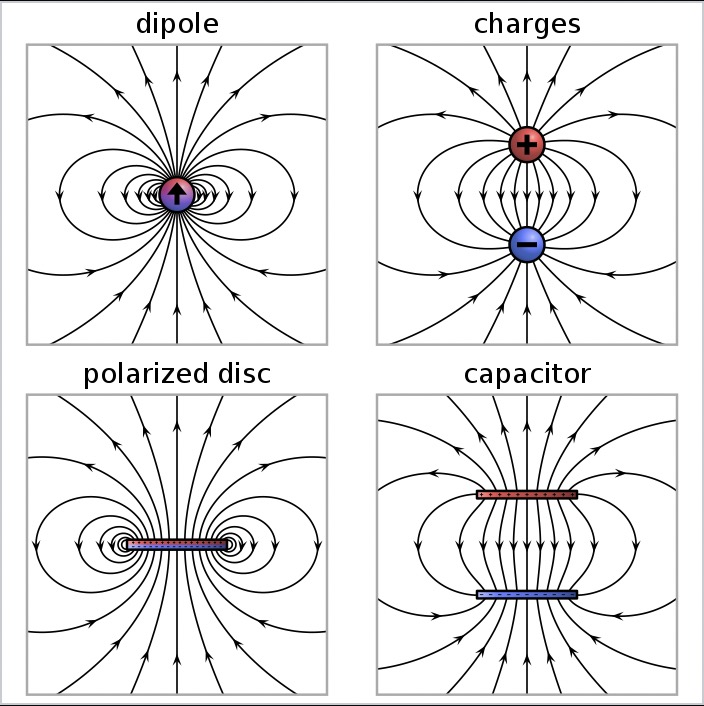
\includegraphics[width=200pt]{final_cheet_sheet_resources/wsqwwfonwjqrkuiumpdthpngngyqovlq.jpg}
\end{section}
\begin{section}{Quiz 2}
 \begin{tabular}{|c|c|}
	 \hline Equation                                                                              & Notes                                                                      \\
	 \hline $\Phi_e = E A \cos \theta = \vec E \cdot A \hat n = \vec E \cdot \vec A$              & $\hat n$ is the normal vector, $\theta$ angle between normal and $\vec E$. \\


	 $\Phi_e = \oint \vec E \cdot d \vec A = \frac{Q_\text{in}}{\epsilon_0}$                      & Gauss' law: Flux through closed surface surrounding charge $q$             \\

	 $\vec E_\text{surface} = \frac{\nu}{\eps}$                                                   & Field at the surface of charged conductor.                                 \\

	 $U_\text{elec} = U_0 + qEs$                                                                  & Potential energy of charge, $U_0$ doesn't matter for $\Delta U$            \\

	 $U = \frac{k q_1 q_2}{r}$                                                                    & Electric potential of system with two point charges.                       \\

	 $U = \sum \frac{k q_i q_j}{r_{ij}}$                                                          & For all pairs $(i,j)$. Num pairs $= \frac{n(n-1)}{2}$                      \\

	 $U_\text{dipole} = - p E \cos \phi = - \vec p \cdot \vec E$                                  & Potential energy of dipole.                                                \\

	 $U_\text{q + sources} = qV$                                                                  & Positive charge slows towards higher potential, speeds up towards lower.   \\

	 $V = Es, E_\text{inside capacitor} = \frac{\Delta V_v}{d}$                                   & Electric potential inside capacitor, $s$ is distance from negative node.   \\

	 $K_f + q V_f = K_i q + V_i$                                                                  & Conservation of energy.                                                    \\

	 $V = \K \frac{Q}{r}$                                                                         & Sphere of charge $r \ge R$                                                 \\

	 $V_\text{ring on axis} = \K \frac{Q}{\sqrt{R^2 + z^2}}$                                      &                                                                            \\

	 $V_\text{disk on axis} = \frac{Q}{2 \pi \epsilon_0 R^2} \left( \sqrt{R^2 + z^2} - z \right)$ &                                                                            \\



	 \hline
 \end{tabular}
 \\
 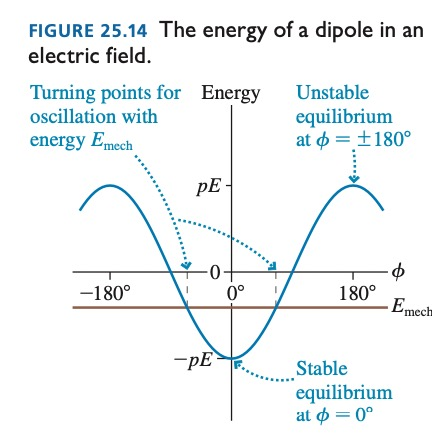
\includegraphics[width=100pt]{final_cheet_sheet_resources/gxmdaouxejjbmynkdouerjsizepbpzqv.jpg}

\end{section}

\begin{section}{Quiz 3}
 \begin{tabular}{|c|c|}
	 \hline
	 Equation                                                                                        & Notes                                                                       \\
	 \hline

	 $V = - \int_{s_i}^{s_f} E \cdot ds, E = - \frac{dV}{ds} \approx - \frac{\Delta V}{\Delta s}   $ &                                                                             \\

	 $\Delta V_\text{loop} = 0 $                                                                     & Kirchhoff's Loop law                                                        \\

	 $Q = C \Delta V_C$                                                                              & C in farads = C/V                                                           \\

	 $C = \frac{Q}{\Delta V_C} = \frac{\eps A}{d}$                                                   & For parallel plate capacitor.                                               \\

	 $C_1 || C_2 = C_1 + C_2, C_1 \perp C_2 = (\frac{1}{C_1} + \frac{1}{C_2})^{-1}$                  & \makecell{Parallel and series capacitors. Series capacitors have equal $Q$, \\ parallel have equal $\Delta V$.} \\

	 $U_C = \frac{Q^2}{2 C} = \frac{1}{2} C (\Delta V_C)^2$                                          & Energy stored in capacitor.                                                 \\
	 $\kappa = \frac{E_0}{E}, \Delta V_C = \frac{(\Delta V_C)_0}{\kappa}, C = \kappa C_0$            & Capacitor with dielectric with constant $\kappa$                            \\

	 \hline
 \end{tabular}
 \\
 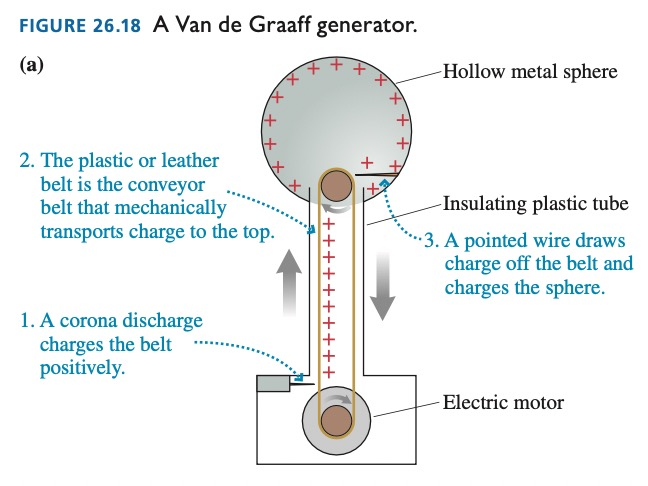
\includegraphics[width=150pt]{final_cheet_sheet_resources/gvotcdmxjpwdvcicmenhqcknyxedpudu.jpg}
 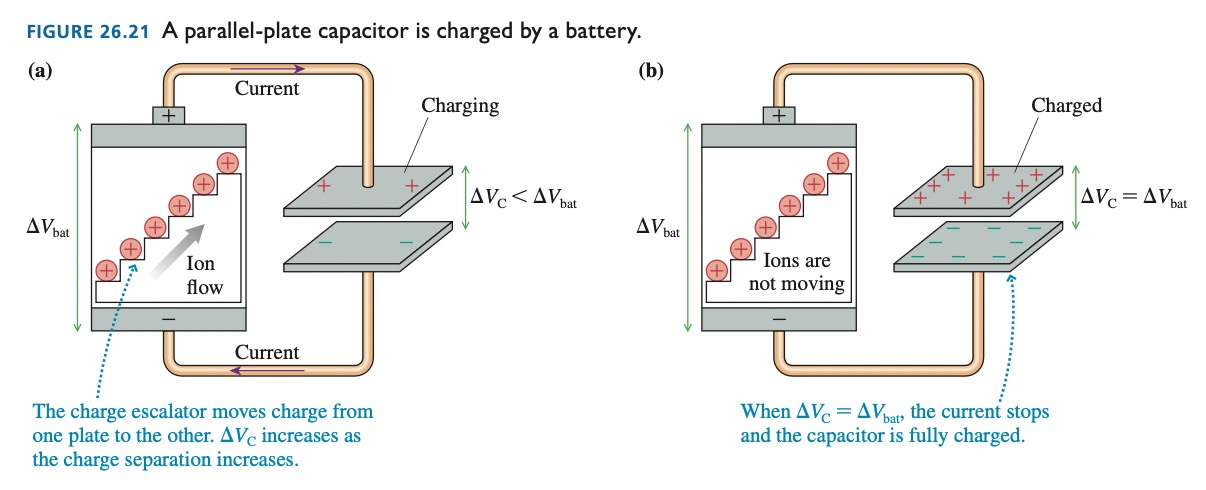
\includegraphics[width=200pt]{final_cheet_sheet_resources/khlzwxxfhkebtizrrtyhiwmbjhtfbalk.jpg}
\end{section}

\begin{section}{Quiz 4}
 \begin{tabular}{|c|c|}
	 \hline
	 Equation                                                                               & Notes                                                               \\
	 \hline
	 $i_e = n_e A v_d$                                                                      & $i_e$ is electron current, $n_e$ electrons/$m^3$, $v_d$ drift speed \\

	 $i_e = \frac{n_e e \tau A}{m} E$                                                       & \makecell{Electron current caused by electric field $E$,            \\ $\tau=$ mean time between collisions. $\frac{1}{\tau}=$ collision rate.} \\

	 $J = \frac{I}{A} = n_e e v_d$                                                          & Current density                                                     \\

	 $\sum I_\text{in} = \sum I_\text{out}$                                                 & Kirchhoff's Junction law.                                           \\

	 $\sigma = \frac{n_e e^2 \tau}{m}, J = \sigma E$                                        & Conductivity and current density                                    \\

	 $\rho = \frac{1}{\sigma}$                                                              & Resistivity.                                                        \\


	 $R = \frac{\rho L}{A}$                                                                 & Resistance in $\Omega \equiv 1 V/A$                                 \\

	 $I = \frac{\Delta V}{R}$                                                               & Ohm's law                                                           \\

	 $R_\text{ideal wire} = 0, R_\text{ideal insulator} = \infty$                           &                                                                     \\

	 $P = \frac{dU}{dt} = \frac{dq}{dt} \mathcal E = I \mathcal E$                          &                                                                     \\

	 $P = I \Delta V_R = I^2 R = \frac{(\Delta V_R)^2}{R}$                                  & Power dissapated by resistor.                                       \\

	 $R_\text{series} = \sum R, R_\text{parallel} = \left( \sum \frac{1}{R_i} \right)^{-1}$ &                                                                     \\

	 $R_\text{ammeter} = 0 \Omega $                                                         & Ideal ammeter                                                       \\

	 $Q = Q_0 e^{-t/RC} = Q_0 e^{-t/\tau}, V = V_0 e^{-t/RC} = V_0 e^{-t/\tau}$             & Charge and voltage across capacitor as it discharges.               \\

	 $Q = Q_0 (1 - e^{-t / \tau}), I = I_0 e^{-t / \tau}$                                   & Capacitor charging                                                  \\

	 $I_\text{cap}(0^+) = I_0, I_\text{cap}(+\infty) = 0$                                   & Capacitor is first a short circuit, approaches closed circuit       \\

	 \hline
 \end{tabular}
 \\
 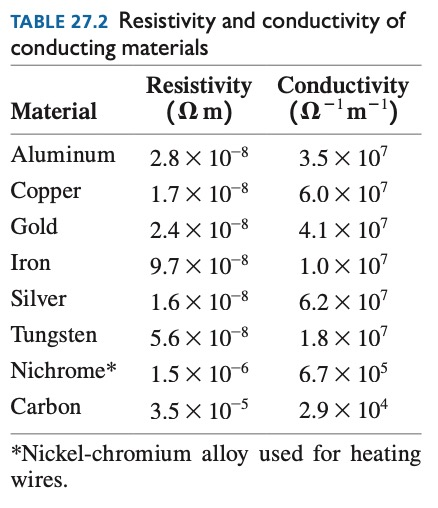
\includegraphics[width=100pt]{final_cheet_sheet_resources/ixfgtziofqygfpdtukouoiqdzfbfaoed.jpg}
\end{section}

\begin{section}{Quiz 5}
 \begin{tabular}{|c|c|}
	 \hline
	 Equation                                                                                                                               & Notes                                                              \\
	 \hline

	 $\vec B_\text{point charge} = \frac{\mu_0}{4 \pi} \frac{qv \sin \theta}{r^2} = \frac{\mu_0}{4 \pi} \frac{q \vec v \times \hat r}{r^2}$ & Biot-savart law. Direction of right hand rule.                     \\

	 1 tesla = 1 T $= 1 \frac{N}{A m}$                                                                                                      & Unit of magnetic field                                             \\

	 $\makecell{B_\text{wire} = \frac{\mu_0}{2 \pi} \frac{I}{r},
	 B_\text{center of current loop} = \frac{\mu_0}{2} \frac{NI}{R},                                                                                                                                             \\
	 B_\text{solenoid} = \frac{\mu_0 N I}{L} = \mu_0 n I  }$                                                                                & N is number of turns, L is length.                                 \\

	 $\vec B = \frac{\mu_0}{2 \pi} \frac{I \Delta \vec s \times \hat r}{r^2}$                                                               & Magnetic field of short current segment                            \\


	 $\vec \mu = AI$                                                                                                                        & Magnetic dipole moment of current loop, from south to north        \\

	 $B_\text{dipole} = \frac{mu_0}{4 \pi} \frac{2 A I}{z^3} = \frac{mu_0}{4 \pi} \frac{2 \vec \mu}{z^3}$                                   & Field of a current loop/dipole on axis of magnetic dipole.         \\

	 $\oint \vec B \cdot d \vec s = \mu_0 I_\text{through}$                                                                                 & Ampere's law                                                       \\

	 $B_\text{inside wire} = \frac{\mu_0 I}{2 \pi R^2} r$                                                                                   & $r < R$                                                            \\

	 $\vec F_\text{on q} = q \vec v \times \vec B = qvB \sin \alpha $                                                                       & \makecell{Force exerted by magnetic field on moving charge.        \\ Direction by right hand rule. }\\

	 $F = qvB = ma_r = \frac{mv^2}{r}$                                                                                                      & Force by cyclotron motion                                          \\

	 $r_\text{cyc} = \frac{mv}{qB}$                                                                                                         & Cyclotron radius                                                   \\

	 $f_\text{cyc} = \frac{qB}{2 \pi m}$                                                                                                    & Cyclotron frequency                                                \\

	 $\Delta V_H = w v_d B = \frac{IB}{tne}$                                                                                                & Hall voltage, w = width of conductor, t = thickness                \\

	 $\vec F_\text{wire} = I \vec l \times \vec B = IlB \sin \alpha$                                                                        & Force on wire in magnetic field. $\vec l$ in direction of current. \\

	 $F_\text{parallel wires} =  \frac{\mu_0 I_1 I_2 l}{2 \pi d}$                                                                           & Attractive if current in same direction, repulsive otherwise.      \\

	 $\vec \tau = \vec \mu \times \vec B$                                                                                                   & Torque on current carrying loop                                    \\
	 \hline
 \end{tabular}
 \\
 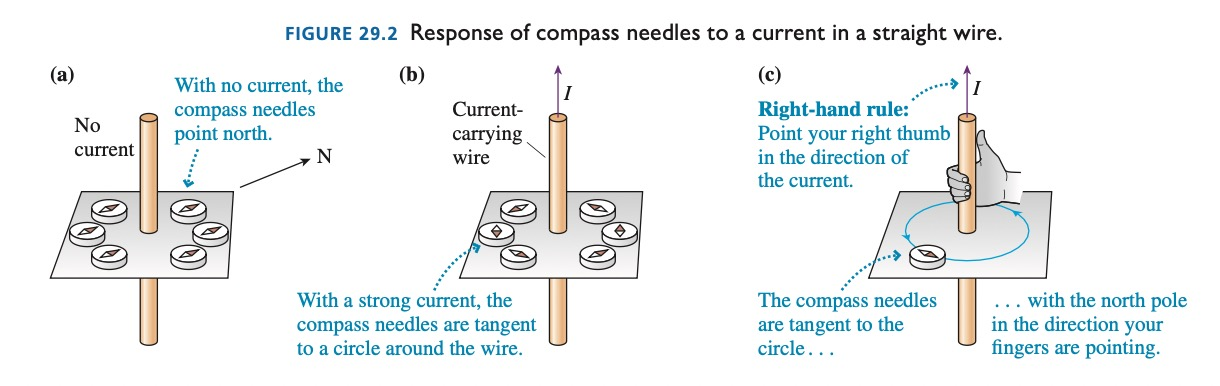
\includegraphics[width=300pt]{final_cheet_sheet_resources/aqszphbxmjmblmaspimhdejdjiugbttc.jpg}
 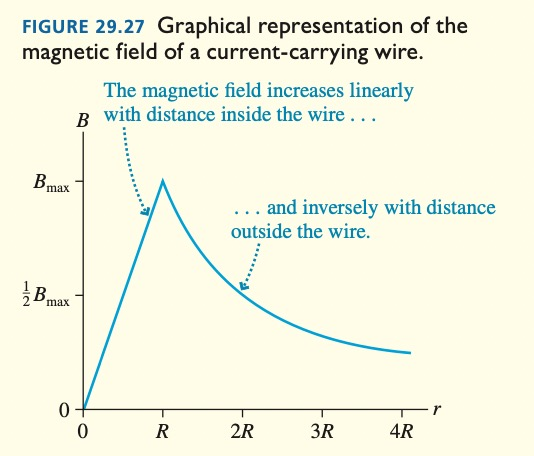
\includegraphics[width=100pt]{final_cheet_sheet_resources/kaozdeuaxhzkquewempuyqchdccgvzoq.jpg}
 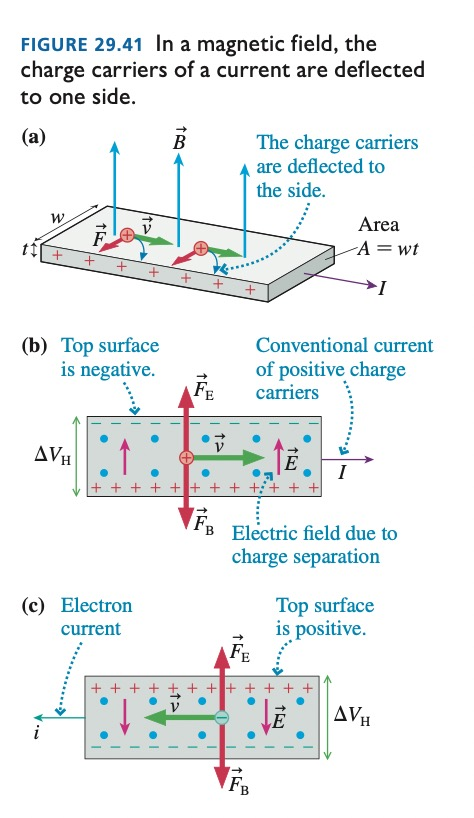
\includegraphics[width=100pt]{final_cheet_sheet_resources/mgsmwhhorrooccpddtidybfkximnvaok.jpg}
\end{section}

\begin{section}{Post-Quiz 5}
 \begin{tabular}{|c|c|}
	 \hline
	 Equation                                                                      & Notes                                                    \\
	 \hline

	 $E = vB$                                                                      & Electric field inside moving conductor in magnetic field \\

	 $\mathcal E = \Delta V = v l B$                                               & Motional emf of conductor moving $\perp$ magnetic field. \\

	 $I = \frac{\mathcal E}{R} = \frac{vlB}{R}$                                    & Current in circuit with moving wire (fig 30.5)           \\

	 $F_\text{pull} = F_\text{mag} = IlB = \frac{vl^2B^2}{R}$                      & Force required to pull the wire at constant speed        \\

	 $P_\text{input} = P_\text{dissapated} = F_\text{pull}v = \frac{v^2l^2B^2}{R}$ & Power in slide wire (generator)                          \\

	 $\Phi_m = AB \cos \theta = \vec A \cdot \vec B $                              & \makecell{Magnetic flux through loop with area. Units in \\
	 weber = 1 Wb = 1 T. $\vec A$ perpendicular to loop. $\text m^2$}                                                                         \\

	 \makecell{There is an induced current iff                                                                                                \\
	 magnetic flux is changing. Direction                                                                                                     \\
	 of current opposes the change.}                                               & Lenz's Law                                               \\

	 $\mathcal E = \oint \vec E \cdot d \vec s =  -\frac{d \Phi_m}{dt} $           & Faraday's law, direction given by Lenz's law             \\

	 $\oint \vec E \cdot d \vec s = A | \frac{dB}{dt} | $                          & Alternative representation of faraday's law              \\

	 $\mathcal E = \frac{\mu_0 A N}{l} | \frac{d I_\text{sol}}{dt} | $             & Induced emf of loop with area $A$ inside solenoid.       \\

	 $E_\text{inside} = \frac{r}{2} | \frac{dB}{dt} |$                             & Field inside solenoid.                                   \\

	 $V_2 = \frac{N_2}{N_1} V_1$                                                   & \makecell{Voltages of a transformer related by           \\ number of turns (fig 30.36).} \\

	 $L = \frac{\Phi_m}{I} = \frac{\mu_0 N^2 A}{l}$                                & Unit henry = 1 H = 1 $\frac{\text{Tm}^2}{A}$             \\

	 $\Delta V_L = -L \frac{dI}{dt}$                                               & \makecell{Potential difference across an                 \\
	 inductor along direction of current.}                                                                                                    \\

	 $U_L = L \int_0^I I dI = \frac{1}{2} L I^2$                                   & Energy stored in inductor                                \\

	 $\omega = \sqrt{\frac{1}{LC}}$                                                & Angular frequency in LC circuit                          \\

	 $Q = Q_0 \cos \omega t$                                                       & Charge of capacitor in LC circuit                        \\

	 $I = - \frac{dQ}{dt} = \omega Q_0 \sin \omega t = I_\text{max} \sin \omega t$ & Current through inductor (LC)                            \\

	 $I = I_0 e^{-t / \tau}, \tau = \frac{L}{R}$                                   & Current in LR circuit                                    \\

	 \hline
 \end{tabular}
 \\
 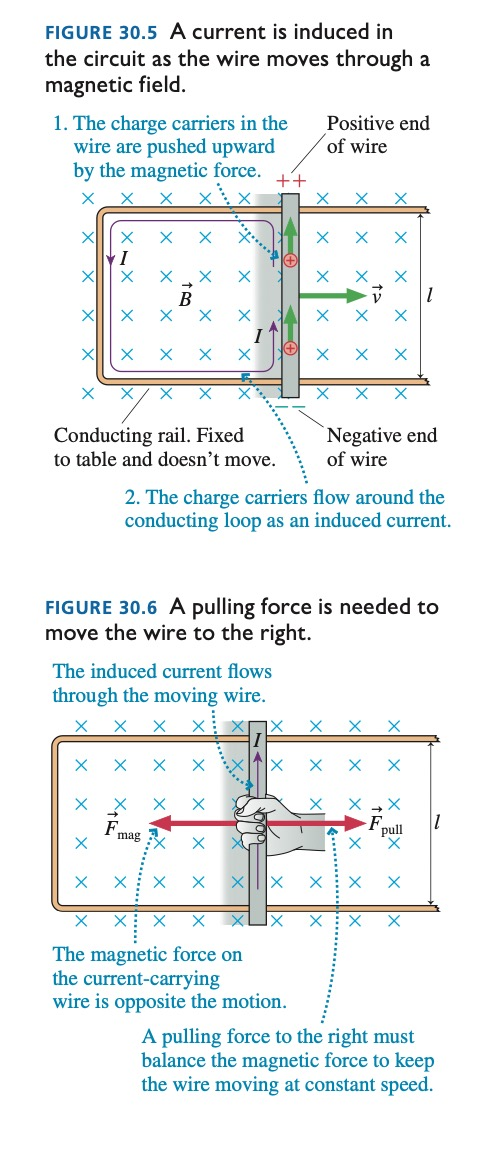
\includegraphics[width=100pt]{final_cheet_sheet_resources/wdvrjkvxydvnmzcxxmvblfduelscmiva.jpg}
 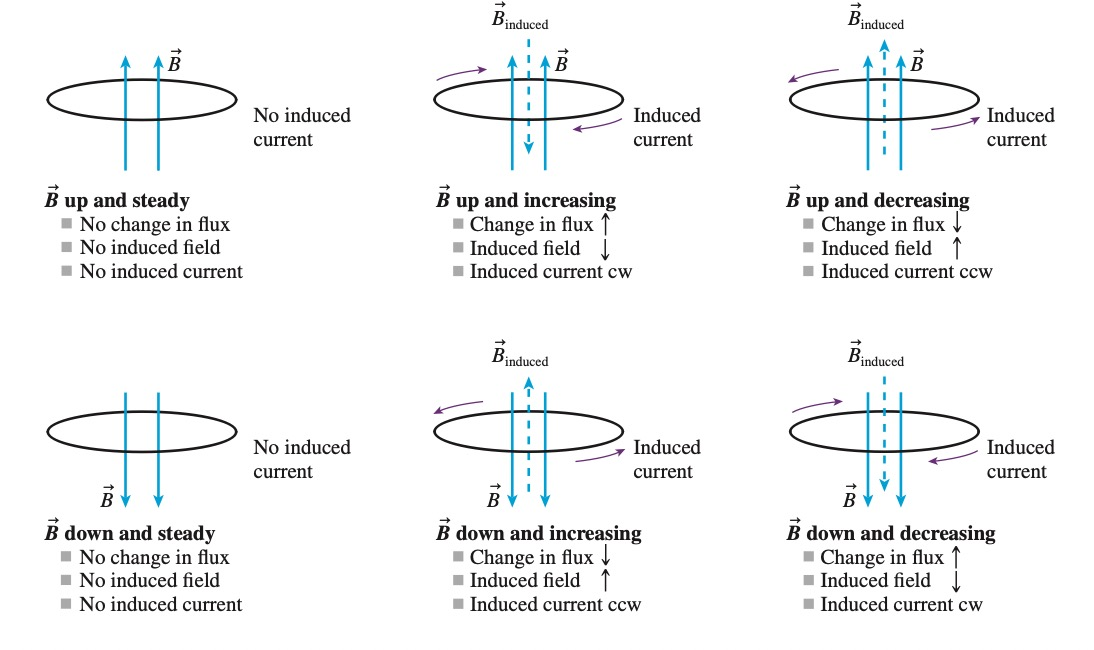
\includegraphics[height=100pt]{final_cheet_sheet_resources/vudruzxbemysxjzyoaltoysmligfugzr.jpg}
 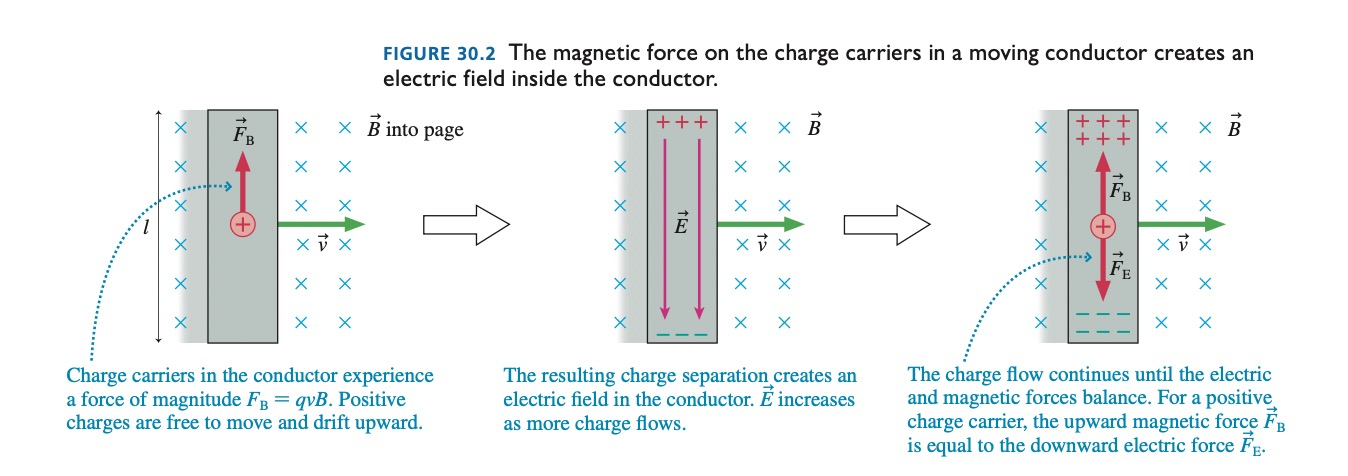
\includegraphics[height=100pt]{final_cheet_sheet_resources/zqygyosdcfxstmovemujxntoqndcyvgs.jpg}
 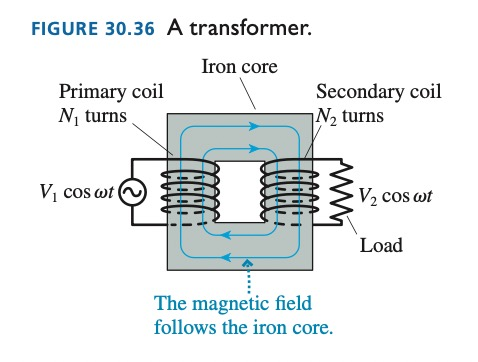
\includegraphics[width=\linewidth]{final_cheet_sheet_resources/tuicoixlhjdxpxepfpdegieiomxwrgca.jpg}
 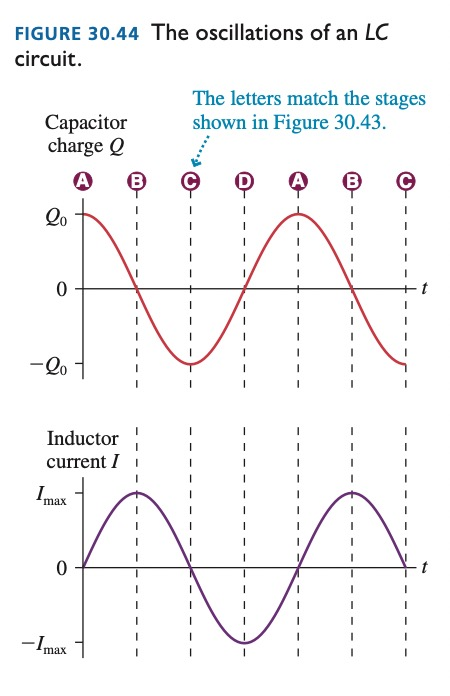
\includegraphics[width=\linewidth]{final_cheet_sheet_resources/knhwzgniatxeirlvrdqvgqrgyvbpycxs.jpg}
\end{section}
\end{document}
